\subsection{Introducción}

En esta sección se implementó un filtro Band-Pass utilizando la aproximación de \textbf{Chebycheff} e implementandola con celdas \textbf{Rauch}. El circuito en cuestión debe cumplir con la siguiente plantilla.
\begin{table}[H]
\centering
\begin{tabular}{|c|c|}
\hline
$Pendiente$      & -40$\frac{dB}{dec}$           \\ \hline
$f_p$      & 28kHz          \\ \hline
$B$      & $\frac{1}{10}$           \\ \hline
$A_p$      & 3dB               \\ \hline
$Filtro$      & BP              \\ \hline
$|Z_{in}|$ & $\geq 50k \Omega$ \\ \hline
\end{tabular}
\caption{Especificaciones del filtro realizado.}
\end{table}

\subsection{Aproximación de Chebycheff.}
Para esta sección se utilizó la aproximación de \textbf{Chebyfeff}. Además, se propuso una plantilla mas restrictiva, con el fin de asegurar el cumplimiento de la original. De esta forma se calculó el valor de $f_p^+$ y $f_p^-$ mediante las ecuaciones
\begin{equation}
	f_0^2 = f_p^+ \cdot f_p^-
\end{equation}
\begin{equation}
	B = \frac{\Delta f_p}{f_0}
\end{equation}

Es así que se obtuvo $f_p^+ =29.435 \ kHz$ y $f_p^- = 26.635 \ kHz$. Luego, teniendo en cuenta que la pendiente originalmente es de 40 dB por década, se tomo una frecuencia de atenuación acorde, tal que mantenga las condiciones de simetría. Es así que se calculó $f_a^+= 294.35 \ kHz$ y $f_a^- = 2.635 \ kHz$.

De esta forma, se obtiene como plantilla final la presentada en la Tabla (\ref{tab:plantilla}).
\begin{table}[H]
\centering
\begin{tabular}{|c|c|}
\hline
$f_s^-$      & 2.6635 kHz          \\ \hline
$f_p^-$      & 26.635 kHz         \\ \hline
$f_p^+$      & 29.435 kHz           \\ \hline
$f_s^+$      & 294.35 kHz          \\ \hline
$A_s$      & 40dB           \\ \hline
$A_p$      & 1dB               \\ \hline
\end{tabular}
\caption{Plantilla cumplida por el filtro.}
\label{tab:plantilla}
\end{table}

Luego, se obtiene la siguiente función transferencia:
\begin{align}
	H(s)=\frac{s\cdot -1.0448\cdot 10^{5}}{s^2+s\cdot 71653+5.2722\cdot 10^{10}}\cdot \frac{s \cdot -74995}{s^2+s\cdot 51101+2.7236 \cdot 10^{10}}
\end{align}

A continuación se plasman los diagramas de ceros y polos de dicho filtro. Estos últimos se caracterizan por poseer un factor $Q$ de 3.23.
\begin{figure}[H]
	\centering
	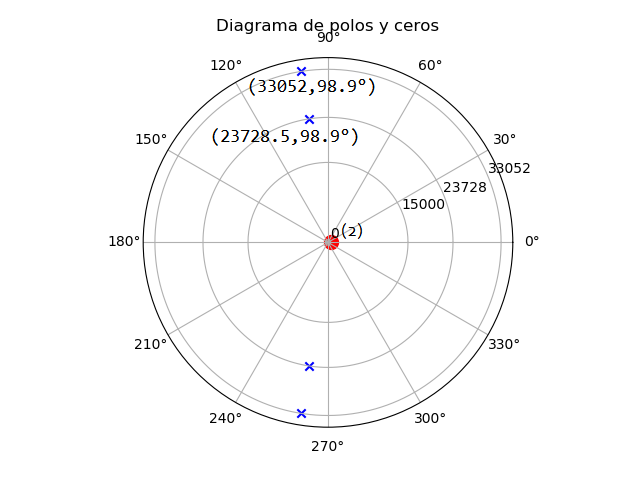
\includegraphics[width=0.5\textwidth]{Imagenes-Ej2/DiagramaPolosYCeros.png}
	\label{fig:stepresponse}
	\caption{Diagrama Polos y Ceros}
\end{figure}

\subsubsection{Elecciones de diseño}
Se decidió armar etapas con celdas segundo orden en cascada, dado a que el orden del filtro es de 4. Para la asociación de polos se tomo criterio, se agrupa cada par con un cero, asociandolos de la siguiente forma.
\begin{figure}[H]
	\centering
	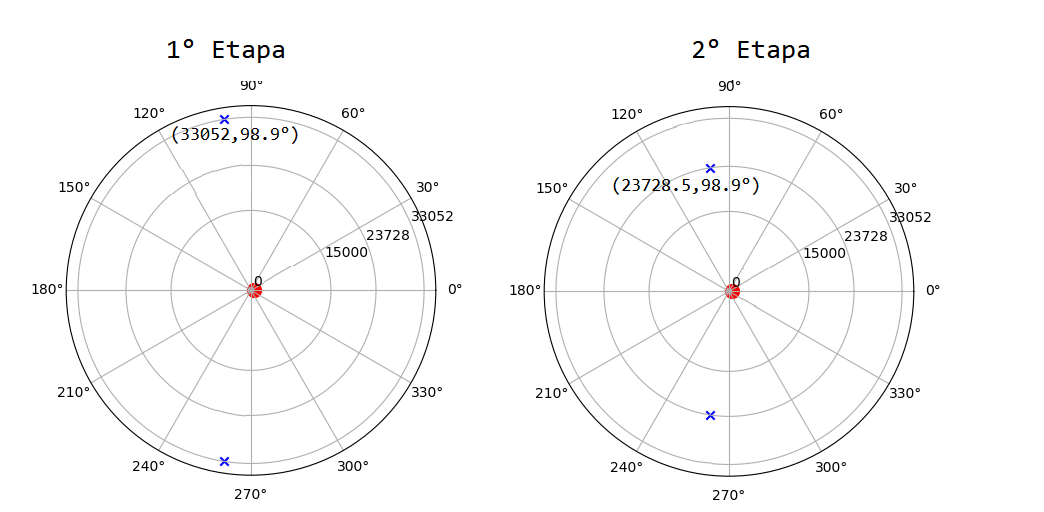
\includegraphics[width=\textwidth]{Imagenes-Ej2/UnionCeros.png}
	\label{fig:CeroPoleUnion}
	\caption{Diagrama de polos y ceros para cada etapa.}
\end{figure}

\subsection{Celda Rauch}
\subsubsection{Cálculo Analítico}
El circuito clásico para una celda 	Rauch pasa-banda (Deliyannis-Friend) es el siguiente:
\begin{figure}[H]
\centering
	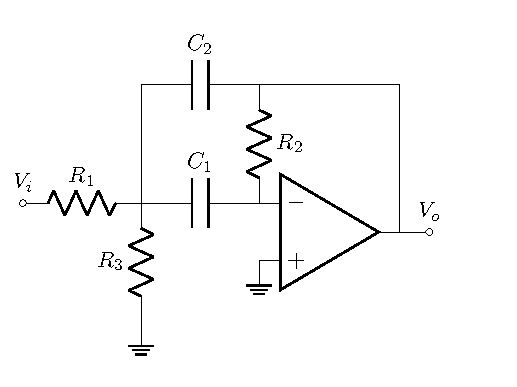
\includegraphics[width=0.55\textwidth, page=1]{Imagenes-Ej2/Circuitos.pdf}
	\caption{Circuito clásico celda Rauch Band-Pass (Deliyannis-Friend).}
	\label{fig:rauch1}
\end{figure}

De aquí, planteando los nodos y considerando el amplificador operacional ideal, se hallan las siguientes ecuaciones:
\begin{equation}
	\frac{V_{in}-V_a}{R_1}+(V_{out}-V_a)\cdot sC_2 -V_a \cdot sC_1 = \frac{V_a}{R_3}
\end{equation}
\begin{equation}
	\frac{V_{out}}{R_2}=-V_a\cdot sC_1
\end{equation}

Con lo planteado previamente, se despeja la función transferencia como:
\begin{align}
H(s)=\frac{s \cdot C_1R_2R_3}{s^2\cdot R_1R_2C_2C_1+s\cdot (C_3R_1R_3+R_1C_2R_3)+R_3+R_1}=\frac{H_0 \cdot \frac{s}{\omega_0 Q}}{\frac{s^2}{\omega_0^2}+\frac{s}{\omega_0Q}+1}
\end{align}

De esta forma, se extraen los parámetros típicos del diseño de filtros siendo los presentados a continuación:
\begin{equation}
	H_0 =\frac{R_2C_2}{R_1C_2+C_1R_1}
\end{equation}
\begin{equation}
	\omega_0^2= \frac{R_1+R_3}{R_1^2R_2C_2C_1}
\end{equation}
\begin{equation}
	Q= \frac{\sqrt[]{1+\frac{R_3}{R_1}}}{{\sqrt[]{\frac{R_3C_1}{R_2C_2}}+\sqrt[]{\frac{R_3C_2}{R_2C_1}}}}
\end{equation}

Luego, para simplificar la elección de componentes, se suele tomar $C_1 = C_2$. De esta forma, para obtener un factor Q relativamente alto, se necesitan valores de resistencias altas, lo cual es un problema. Para solucionarlo, se modificó la celda, incluyendo una realimentación positiva, permitiendo obtener un Q de mayor valor. Finalmente, la celda Rauch con Q mejorado, se presenta a continuación.
\begin{figure}[H]
	\centering
	\includegraphics[width=0.55\textwidth, page=2]{Imagenes-Ej2/Circuitos.pdf}
	\caption{Circuito celda Rauch Band-Pass con Q mejorado.}	
	\label{fig:rauch2}	
\end{figure}

Para resolver el circuito presentado en la Figura (\ref{fig:rauch2}), basta con plantear los siguientes nodos:
\begin{equation}
	\frac{V_{out}-K \cdot V_{out}}{R_2}=(K \cdot V_{out}-V_a)\cdot sC_1
\end{equation}
\begin{equation}
	\frac{V_{in}-V_a}{R_1}+(V_{out}-V_a)\cdot sC_2 +(K \cdot V_{out}-V_a) \cdot sC_1 = \frac{V_a}{R_3}
\end{equation}

Es así que se obtiene la transferencia del circuito, siendo esta la presentada a continuación.
\begin{align}
H(s)=\frac{1}{1-K} \cdot \frac{H_0 \cdot \frac{s}{\omega_0 Q_0}}{\frac{s^2}{\omega_0^2}+\frac{s}{\omega_0Q}+1}
\end{align}

De ella se obtiene $Q_0$, la cual es una constante de valor 1.5\footnote{R. Schaumann, H. Xiao, M. Van Valkenburg, M. Van Valkenburg and M. Van Valkenburg, Analog filter design. New York: Oxford University Press, 2011, pp. 170-176.}, y el K es utilizado para ajustar el valor de Q del circuito, dado que quedarán así definidos los parámetros del filtro:
\begin{align}
\omega_0^2= \frac{R_1+R_3}{R_1R_3R_2C_2C_1}
\label{eq:omeg}
\end{align}
\begin{align}
Q=\frac{Q_0}{1-2Q_0^2\cdot \frac{K}{1-K}}=\frac{\sqrt[]{R_1R_3R_2C_1C_2(R_1+R_3)}}{R_1R_3(C_1+C_2)-\frac{K}{1-K}(R_1+R_3)R_2C_1}
\label{eq:Q}
\end{align}
\begin{align}
H_0=\frac{R_3R_2}{(C_1+C_2)\cdot (K-1)R_1R_3+K(R_1+R_3)R_2 C_2}
\label{eq:H0}
\end{align}
También es posible calcular la impedancia de entrada de la celda. 
\begin{align}
Z_{in}(s)=\frac{V_{in}(s)}{I_{in}(s)}= \frac{s^2 R_1R_2R_3C_1C_2+s\cdot R_1R_3(C_1+C_2)+R_1+R_3}{s^2R_3R_2C_1C_2+sR_3(C_1+C_2)+1}
\end{align}

\subsubsection{Elecciones de diseño}
Se realiza el cálculo de sensibilidades a partir de las expresiones (\ref{eq:omeg}), (\ref{eq:Q}) y (\ref{eq:H0}), obteniéndose así las expresiones presentadas en las Tablas (\ref{tab:senswyg}) y (\ref{tab:sesq}).
\begin{table}[H]
\centering
\begin{tabular}{ccc}
\hline
Componente & $S^{\omega_0}$ & $S^{H_0}$ \\ \cline{1-3}\\
$S_{R_1}$  & $-{\frac {{\it R3}}{ 2.0\,{\it R1}+ 2.0\,{\it R3}}}$    &$ -{\frac { \left( {\it C1}\,K{\it R3}+K{\it R2}\,{\it C2}+{\it C2}\,K{
\it R3}-{\it C1}\,{\it R3}-{\it C2}\,{\it R3} \right) {\it R1}}{{\it 
C1}\,K{\it R1}\,{\it R3}+K{\it R2}\,{\it C2}\,{\it R1}+{\it C2}\,K{
\it R1}\,{\it R3}+K{\it R2}\,{\it C2}\,{\it R3}-{\it C1}\,{\it R1}\,{
\it R3}-{\it C2}\,{\it R1}\,{\it R3}}} $  \\
$S_{R_2}$  & -0.5    & ${\frac {{\it R1}\,{\it R3}\, \left( {\it C1}\,K+{\it C2}\,K-{\it C1}-{
\it C2} \right) }{{\it C1}\,K{\it R1}\,{\it R3}+K{\it R2}\,{\it C2}\,{
\it R1}+{\it C2}\,K{\it R1}\,{\it R3}+K{\it R2}\,{\it C2}\,{\it R3}-{
\it C1}\,{\it R1}\,{\it R3}-{\it C2}\,{\it R1}\,{\it R3}}}$   \\
$S_{R_3}$  & $-{\frac {{\it R1}}{ 2.0\,{\it R1}+ 2.0\,{\it R3}}}$     & ${\frac {K{\it R2}\,{\it C2}\,{\it R1}}{{\it C1}\,K{\it R1}\,{\it R3}+K
{\it R2}\,{\it C2}\,{\it R1}+{\it C2}\,K{\it R1}\,{\it R3}+K{\it R2}\,
{\it C2}\,{\it R3}-{\it C1}\,{\it R1}\,{\it R3}-{\it C2}\,{\it R1}\,{
\it R3}}}$   \\
$S_{C_1}$  & -0.5    & $-{\frac {{\it R3}\,{\it R1}\, \left( -1+K \right) {\it C1}}{{\it C1}\,
K{\it R1}\,{\it R3}+K{\it R2}\,{\it C2}\,{\it R1}+{\it C2}\,K{\it R1}
\,{\it R3}+K{\it R2}\,{\it C2}\,{\it R3}-{\it C1}\,{\it R1}\,{\it R3}-
{\it C2}\,{\it R1}\,{\it R3}}}$  \\
$S_{C_2}$  & -0.5    & $-{\frac { \left( K{\it R2}\,{\it R1}+{\it R1}\,{\it R3}\,K+K{\it R2}\,
{\it R3}-{\it R1}\,{\it R3} \right) {\it C2}}{{\it C1}\,K{\it R1}\,{
\it R3}+K{\it R2}\,{\it C2}\,{\it R1}+{\it C2}\,K{\it R1}\,{\it R3}+K{
\it R2}\,{\it C2}\,{\it R3}-{\it C1}\,{\it R1}\,{\it R3}-{\it C2}\,{
\it R1}\,{\it R3}}}$ \\
\hline
\end{tabular}
\caption{Tabla de sensibilidades de $\omega_0$ y de la ganancia.}
\label{tab:senswyg}
\end{table}
\begin{table}[H]
\centering
\begin{tabular}{cc}
\hline
Componente & $S^{Q}$ \\ \hline\\
$S_{R_1}$  & $1/2\,{\frac {{\it R3}\, \left( K{\it R2}\,{\it C1}\,{\it R1}-{\it C1}
\,K{\it R1}\,{\it R3}+K{\it R2}\,{\it C1}\,{\it R3}-{\it C2}\,K{\it R1
}\,{\it R3}+{\it C1}\,{\it R1}\,{\it R3}+{\it C2}\,{\it R1}\,{\it R3}
 \right) }{ \left( K{\it R2}\,{\it C1}\,{\it R1}+{\it C1}\,K{\it R1}\,
{\it R3}+K{\it R2}\,{\it C1}\,{\it R3}+{\it C2}\,K{\it R1}\,{\it R3}-{
\it C1}\,{\it R1}\,{\it R3}-{\it C2}\,{\it R1}\,{\it R3} \right) 
 \left( {\it R1}+{\it R3} \right) }}$ \\
$S_{R_2}$  & $-1/2\,{\frac {K{\it R2}\,{\it C1}\,{\it R1}-{\it C1}\,K{\it R1}\,{\it 
R3}+K{\it R2}\,{\it C1}\,{\it R3}-{\it C2}\,K{\it R1}\,{\it R3}+{\it 
C1}\,{\it R1}\,{\it R3}+{\it C2}\,{\it R1}\,{\it R3}}{K{\it R2}\,{\it 
C1}\,{\it R1}+{\it C1}\,K{\it R1}\,{\it R3}+K{\it R2}\,{\it C1}\,{\it 
R3}+{\it C2}\,K{\it R1}\,{\it R3}-{\it C1}\,{\it R1}\,{\it R3}-{\it C2
}\,{\it R1}\,{\it R3}}}$ \\
$S_{R_3}$  & $1/2\,{\frac {{\it R1}\, \left( K{\it R2}\,{\it C1}\,{\it R1}-{\it C1}
\,K{\it R1}\,{\it R3}+K{\it R2}\,{\it C1}\,{\it R3}-{\it C2}\,K{\it R1
}\,{\it R3}+{\it C1}\,{\it R1}\,{\it R3}+{\it C2}\,{\it R1}\,{\it R3}
 \right) }{ \left( K{\it R2}\,{\it C1}\,{\it R1}+{\it C1}\,K{\it R1}\,
{\it R3}+K{\it R2}\,{\it C1}\,{\it R3}+{\it C2}\,K{\it R1}\,{\it R3}-{
\it C1}\,{\it R1}\,{\it R3}-{\it C2}\,{\it R1}\,{\it R3} \right) 
 \left( {\it R1}+{\it R3} \right) }}$ \\
$S_{C_1}$  & $-1/2\,{\frac {K{\it R2}\,{\it C1}\,{\it R1}+{\it C1}\,K{\it R1}\,{\it 
R3}+K{\it R2}\,{\it C1}\,{\it R3}-{\it C2}\,K{\it R1}\,{\it R3}-{\it 
C1}\,{\it R1}\,{\it R3}+{\it C2}\,{\it R1}\,{\it R3}}{K{\it R2}\,{\it 
C1}\,{\it R1}+{\it C1}\,K{\it R1}\,{\it R3}+K{\it R2}\,{\it C1}\,{\it 
R3}+{\it C2}\,K{\it R1}\,{\it R3}-{\it C1}\,{\it R1}\,{\it R3}-{\it C2
}\,{\it R1}\,{\it R3}}}$ \\
$S_{C_2}$  & $1/2\,{\frac {K{\it R2}\,{\it C1}\,{\it R1}+{\it C1}\,K{\it R1}\,{\it 
R3}+K{\it R2}\,{\it C1}\,{\it R3}-{\it C2}\,K{\it R1}\,{\it R3}-{\it 
C1}\,{\it R1}\,{\it R3}+{\it C2}\,{\it R1}\,{\it R3}}{K{\it R2}\,{\it 
C1}\,{\it R1}+{\it C1}\,K{\it R1}\,{\it R3}+K{\it R2}\,{\it C1}\,{\it 
R3}+{\it C2}\,K{\it R1}\,{\it R3}-{\it C1}\,{\it R1}\,{\it R3}-{\it C2
}\,{\it R1}\,{\it R3}}}$ \\
\hline
\end{tabular}
\caption{Tabla de sensibilidades de Q.}
\label{tab:sesq}
\end{table}

Reemplazando por valores numéricos en las expresiones presentadas anteriormente, se obtienen los valores presentados en las Tablas (\ref{tab:ses1}) y (\ref{tab:ses2}).
\begin{table}[H]
\centering
\begin{tabular}{cccc}
\hline
\multicolumn{4}{c}{Etapa 1}                                                                      \\ \hline
Componente                    & $S^{H_0}$               & $S^{Q}$               & $S^{\omega_0}$ \\ \hline
$S_{R_1}$                     & -1.33                   & -0.41                 & -0.08          \\
$S_{R_2}$                     & 3                       & 2.5                   & -0.5           \\
$S_{R_3}$                     & -1.67                   & -2.09                 & -0.45          \\
$S_{C_1}$                     & -1.5                    & -1                    & -0.5           \\
$S_{C_2}$ & 1.5 & 1 & -0.5        \\
\hline  
\end{tabular}
\caption{Tabla de sensibilidades de la primer etapa.}
\label{tab:ses1}
\end{table}
\begin{table}[H]
\centering
\begin{tabular}{cccc}
\hline
\multicolumn{4}{c}{Etapa 1}                                                                      \\ \hline
Componente                    & $S^{H_0}$               & $S^{Q}$               & $S^{\omega_0}$ \\ \hline
$S_{R_1}$                     & -1.33                   & -0.41                 & -0.08          \\
$S_{R_2}$                     & 3                       & 2.5                   & -0.5           \\
$S_{R_3}$                     & -1.67                   & -2.09                 & -0.42          \\
$S_{C_1}$                     & -1.5                    & -1                    & -0.5           \\
$S_{C_2}$ & 1.5 & 1 & -0.5        \\
\hline  
\end{tabular}
\caption{Tabla de sensibilidades de la segunda etapa.}
\label{tab:ses2}
\end{table}

En base a lo establecido en las tablas previas, se tomó especial cuidado en la elección de componentes y en el matcheo de impedancias. De esta forma, los componentes utilizados son los siguientes:
\begin{table}[H]
\centering
\begin{tabular}{ccccc}
\hline
\multicolumn{1}{c}{Componente} & \multicolumn{1}{c}{1er Etapa} & \multicolumn{1}{c}{Composición} & 2da Etapa      & Composición           \\ \hline
$R_1$                          & $7.3 k\Omega$                 & $10k // 27k  \Omega$            & $5.24 k\Omega$ & $5.6k // 82k  \Omega$ \\
$R_2$                          & $5.56 k\Omega$                & $5.6k // 680k  \Omega$          & $3.99 k\Omega$ & $82 + 3.9k  \Omega$   \\
$R_3$                          & $1.43 k\Omega$                & $1.5 k // 33k  \Omega$          & $1.03k\Omega$  & $27 + 1k  \Omega$     \\
$R_4$                          & $3.49 k\Omega$                & $3.9k // 33k  \Omega$           & $3.49 k\Omega$ & $3.9k // 33k  \Omega$ \\
$R_5$                          & $1 k\Omega$                   & $1 k  \Omega$                   & $1 k\Omega$    & $1 k\Omega$           \\
$C_1$                          & 2.35 nF         & (4.7+4.7) nF                          & 2.35 nF         & (4.7+4.7) nF                \\
$C_2$                          & 2.35 nF         & (4.7+4.7) nF                          & 2.35 nF         & (4.7+4.7) nF               \\
\hline
\end{tabular}
\caption{Componentes seleccionados para el filtro.}
\end{table}

Luego, se calculó el error porcentual asociado a la aproximación de la resistencias, expresando los resultados obtenidos en la Tabla (\ref{tab:error}).
\begin{table}[H]
\centering
\begin{tabular}{ccc}
\hline
\multicolumn{1}{c}{Error Porcentual} & \multicolumn{1}{c}{1er Etapa} & \multicolumn{1}{c}{2da Etapa} \\ \hline
$R_1$                                & 0.1 $\%$                      & $0.038  \%$                   \\
$R_2$                                & 0.1 $\%$                      & 0.2 $\%$                      \\
$R_3$                                & 0.4 $\%$                      & 0.1 $\%$                      \\
$R_4$                                & 0.1 $\%$                      & 0.1 $\%$                      \\
$R_5$                                & $\approx 0 \%$                & $\approx 0 \%$                \\
$C_1$                                & $\approx 0 \%$                & $\approx 0 \%$                \\
$C_1$                                & $\approx 0 \%$                & $\approx 0 \%$            \\
\hline
\end{tabular}
\caption{Error porcentual de los componetnes.}
\label{tab:error}
\end{table}

Cabe destacar que todas las impedancias que fueron colocadas en el circuito fueron elegidas entre varias de su mismo tipo, ya que estas fueron medidas, garantizando así que las utilizadas sean realmente de los valores deseados.

\subsubsection{Acoplamiento de Impedancias}

Para que ambas etapas no se carguen entre, la impedancia de entrada de la segunda etapa debe ser mucho mayor a la de salida de la primera. Para garantizar que ello ocurra, se simularon las impedancias de entrada de ambas celdas, incluyendo la de salida de la primera.
\begin{figure}[H]
	\centering
	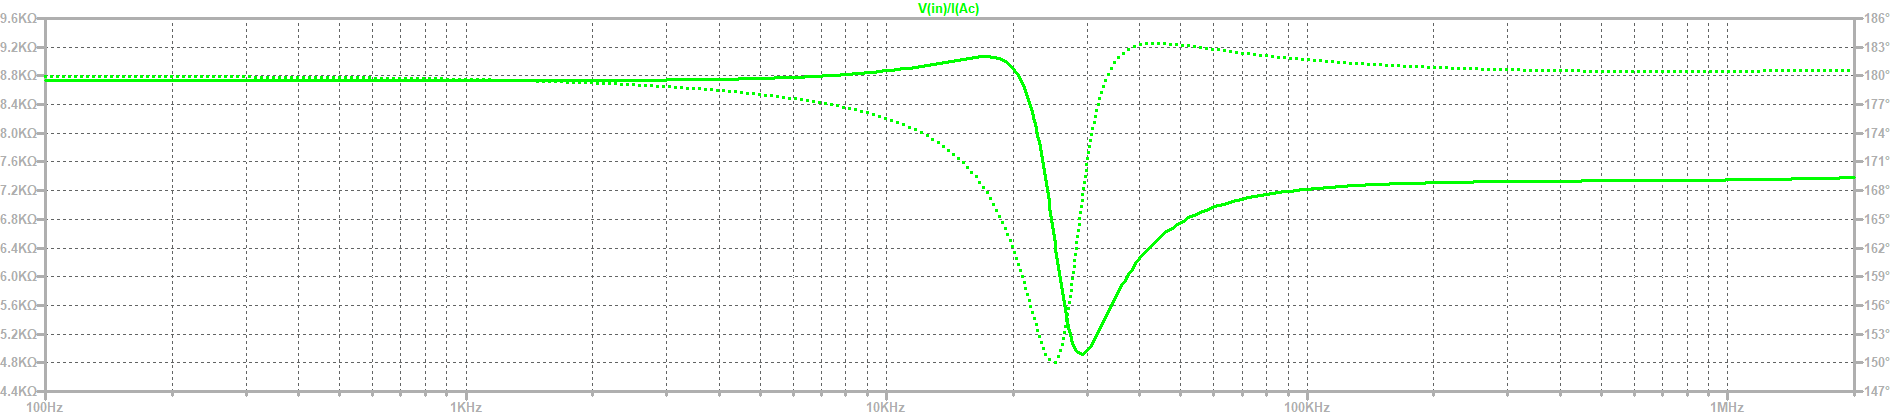
\includegraphics[width=\textwidth]{Imagenes-Ej2/ZinE1.png}
	\label{fig:graph}
	\caption{Impedancia de entrada de la primer etapa.}
\end{figure}
\begin{figure}[H]
	\centering
	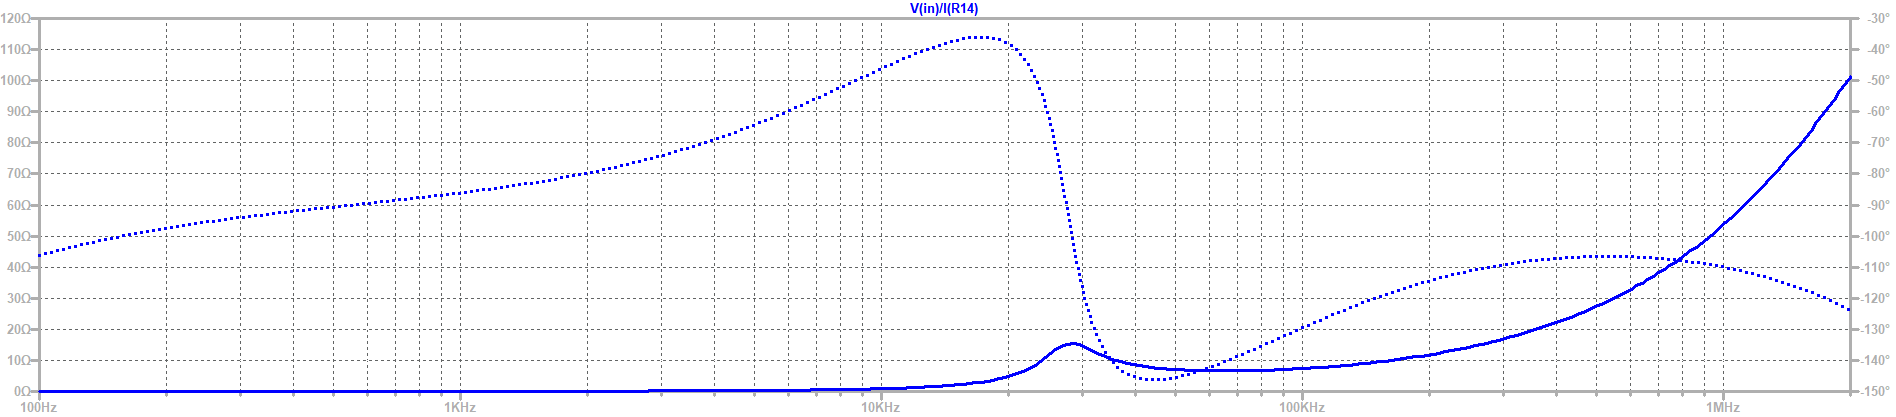
\includegraphics[width=\textwidth]{Imagenes-Ej2/ZoutE1.png}
	\label{fig:graph}
	\caption{Impedancia de salida de la primer etapa.}
\end{figure}
\begin{figure}[H]
	\centering
	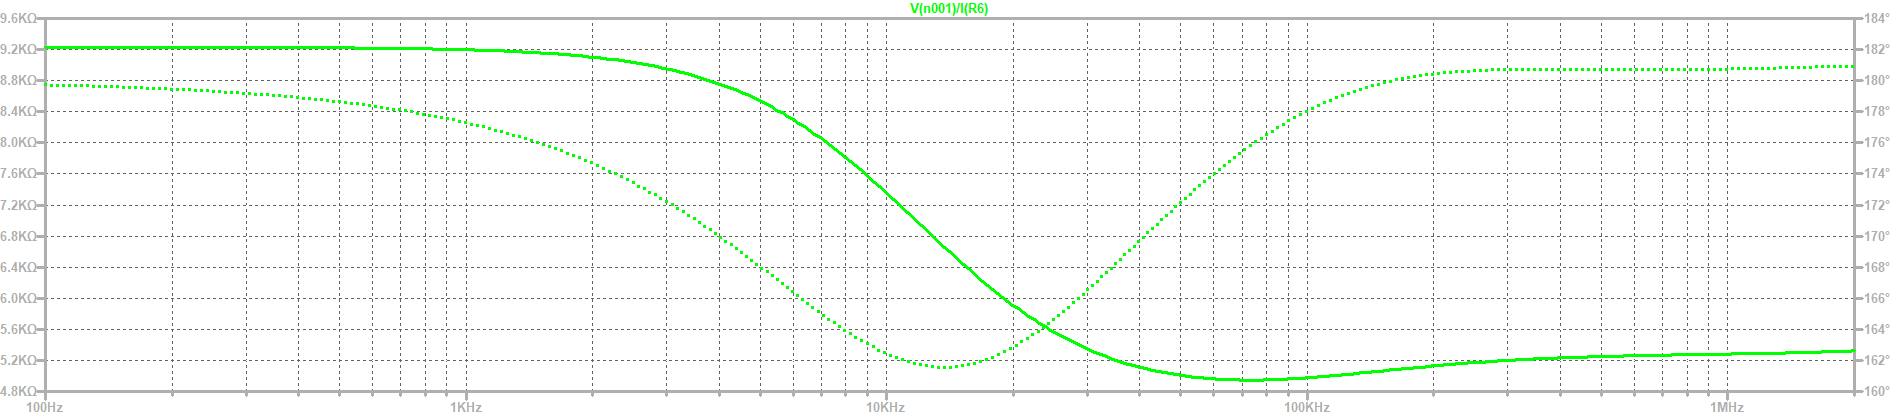
\includegraphics[width=\textwidth]{Imagenes-Ej2/ZinE2.png}
	\label{fig:graph}
	\caption{Impedancia de entrada de la segunda etapa.}
\end{figure}

Se puede apreciar que la impedancia de salida de la primer etapa es mucho menor en comparación a la de entrada de la segunda, por lo tanto, se da un buen acoplamiento de impedancias y no es necesario el uso de buffers.

\subsection{Respuesta en Frecuencia}
Se realizó un análisis de Montecarlo de la respuesta en frecuencia del circuito, utilizando una tolerancia de las resistencias al $1\%$ y capacitores al $10\%$ obteniendo la siguiente dispersión.
\begin{figure}[H]
	\centering
	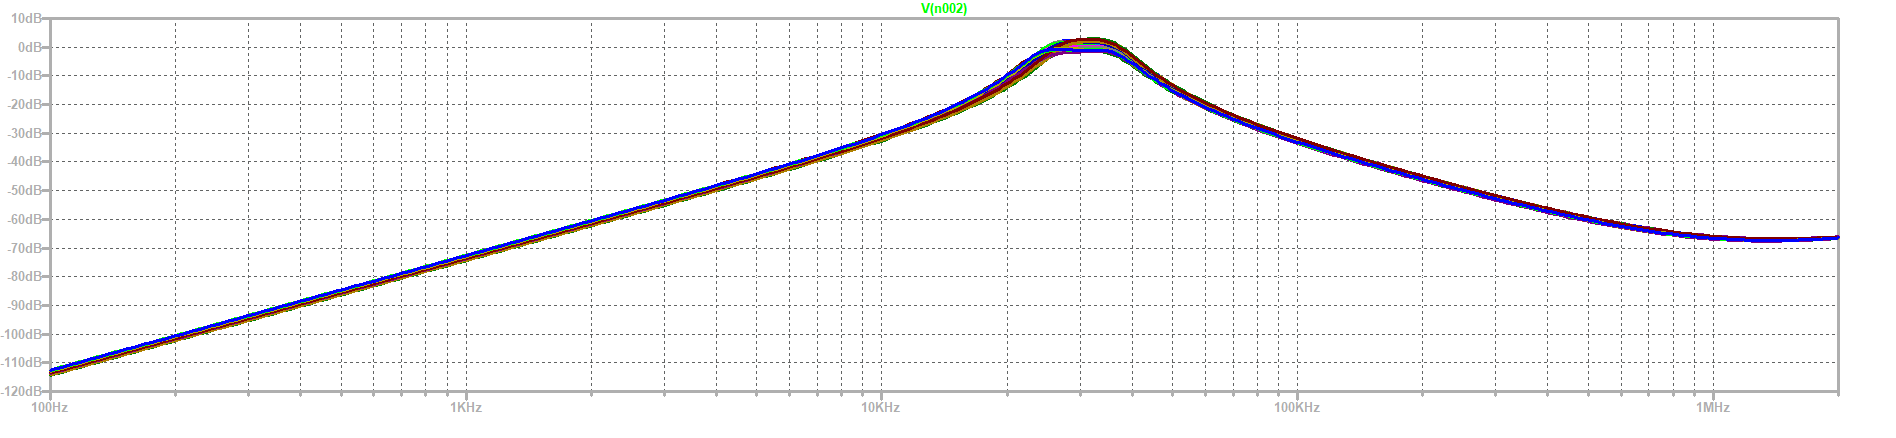
\includegraphics[width=\textwidth]{Imagenes-Ej2/mcF.png}
	\caption{Análisis de Montecarlo del filtro.}
	\label{fig:mcrauch}
\end{figure}

\subsection{Rango Dinámico.}
El rango dinámico se define como la razón entre el máximo y mínimo valor que puede tomar un observable de interés. Para el caso en cuestión, queda definido de la forma
\begin{align}
R_d = 20 \log_{10} \left( \frac{V_{in_{max}}}{V_{in_{min}}} \right)
\end{align}

Para definir $V_{in_{min}}$, se tuvo en cuenta la tensión mínima que se pudo distinguir respecto al piso de ruido, la cual es de $V_{in_{min}} \approx 10 \ mV$. Luego, para el caso de $V_{in_{max}}$, se tuvo en cuenta la máxima tensión previa a la aparición de alinealidades, siendo estos efectos el cross-over, slew-rate y saturación del amplificador operacional. Dos de estos problemas son solucionados mediante la elección del integrado, ya que se utiliza un TL081, el cual tiene un slew-rate elevado y no posee el problema del cross-over debido a su etapa de salida. Por su parte, para el problema de la saturación, es de utilidad saber que la máxima tensión de salida es $V_{sat} = Vcc - 1.5 \ V = 13.5 \ V$. Para encontrar el valor de tensión máximo de entrada se consideró la ganancia del sistema y, teniendo en cuenta la conexión entre etapas, este factor queda definido por la siguiente expresión:
\begin{align}
V_{in_{max}}=\frac{V_{sat}}{  \max(G_{E1} \cdot G_{E2} )} = 12.24V
\end{align}
Es así que con lo mencionado previamente, se obtiene $R_d = 61.75dB$.

\subsubsection{Etapas}
Se realizaron 2 etapas, ambas siendo el mismo tipo de celda, pero con distintos parámetros. Para cada una, se decidió realizar un análisis de Montecarlo
\begin{figure}[H]
	\centering
	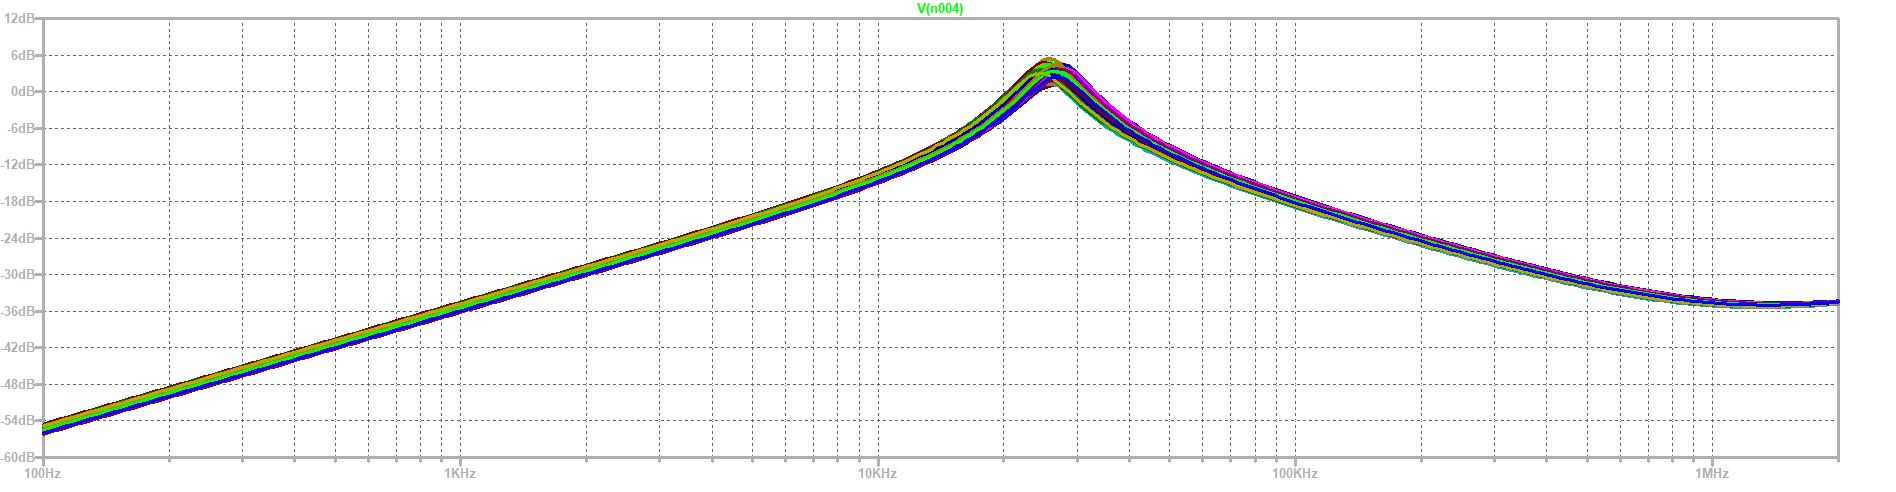
\includegraphics[width=\textwidth]{Imagenes-Ej2/mcE1.png}
	\caption{Análisis de Montecarlo de la primer etapa.}
	\label{fig:mc1}
\end{figure}
\begin{figure}[H]
	\centering
	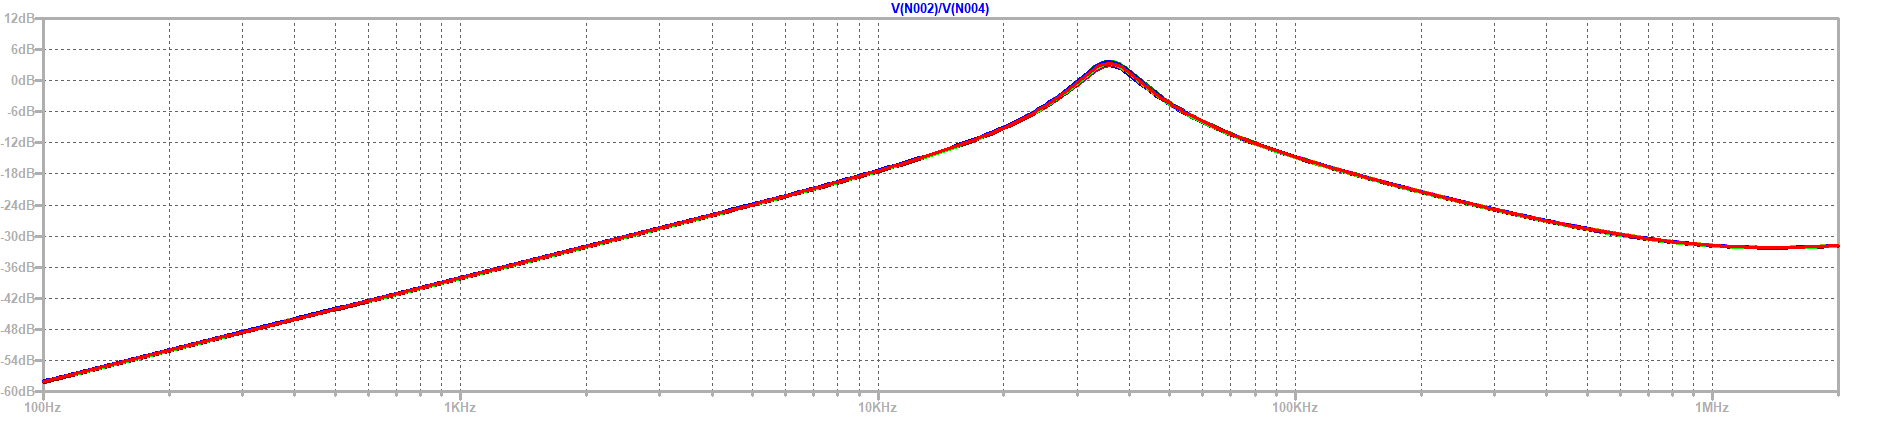
\includegraphics[width=\textwidth]{Imagenes-Ej2/mcE2.png}
	\caption{Análisis de Montecarlo de la segunda etapa.}
	\label{fig:mc2}
\end{figure}

Es notable que no existe una gran dispersión debido a los componentes en el diagrama de bode. Más allá de esto, mirando las sensibilidades, se nota una gran dependencia, tanto en el Q como en la frecuencia de corte del sistema, con respecto a la resistencia $R_3$. Es por ello que a continuación se presentan dos simulaciones de Montecarlo. Una representa la variación de dicha resistencia en cada etapa, mientras que la otra muestra como afecta cada una al filtro final.

Primero se presenta la variación de $R_3$ en la primer etapa, modificandola entre $100 \ \Omega$ y $2 \ k\Omega$.  
\begin{figure}[H]
	\centering
	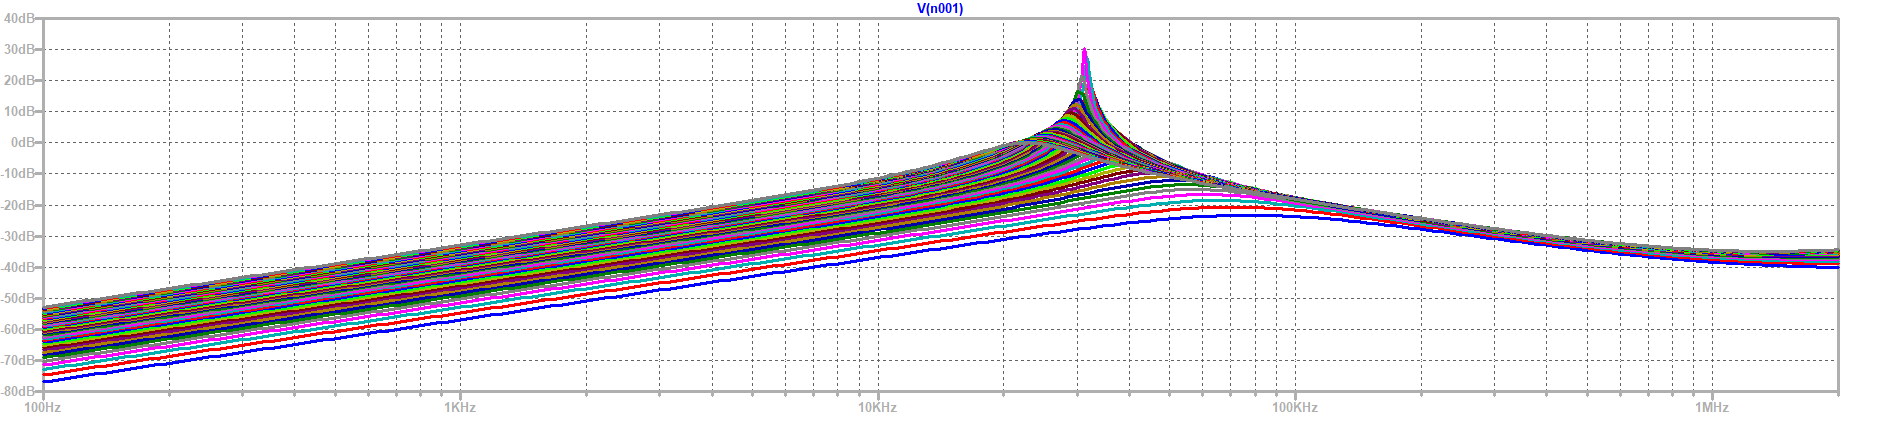
\includegraphics[width=\textwidth]{Imagenes-Ej2/presetE1.png}
	\label{fig:mcr3-1}
	\caption{Variación salida de la primer etapa al cambiar $R_3$.}
\end{figure}
\begin{figure}[H]
	\centering
	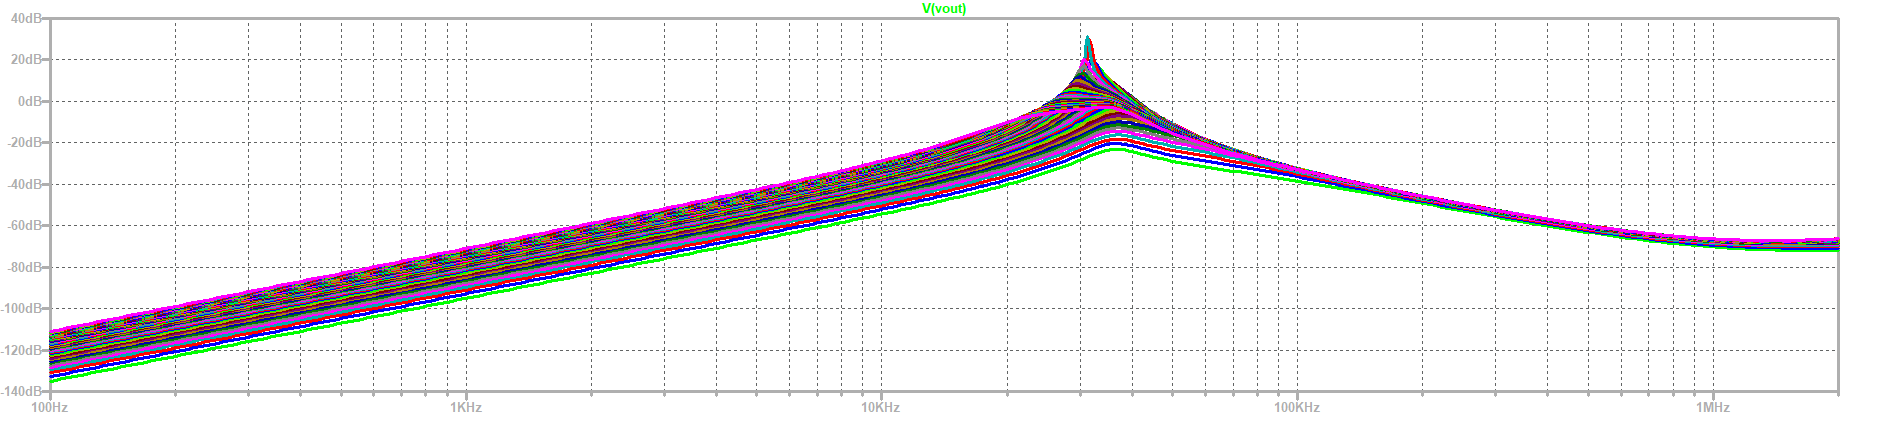
\includegraphics[width=\textwidth]{Imagenes-Ej2/presetEFE1.png}
	\label{fig:graph}
	\caption{Variación salida del filtro al cambiar $R_3$ de la primer etapa.}
\end{figure}

Se puede notar como se modifica el Q del circuito al igual que el valor de la frecuencia de corte. Luego se prosiguió a realizar el mismo análisis, pero de la siguiente etapa.
\begin{figure}[H]
	\centering
	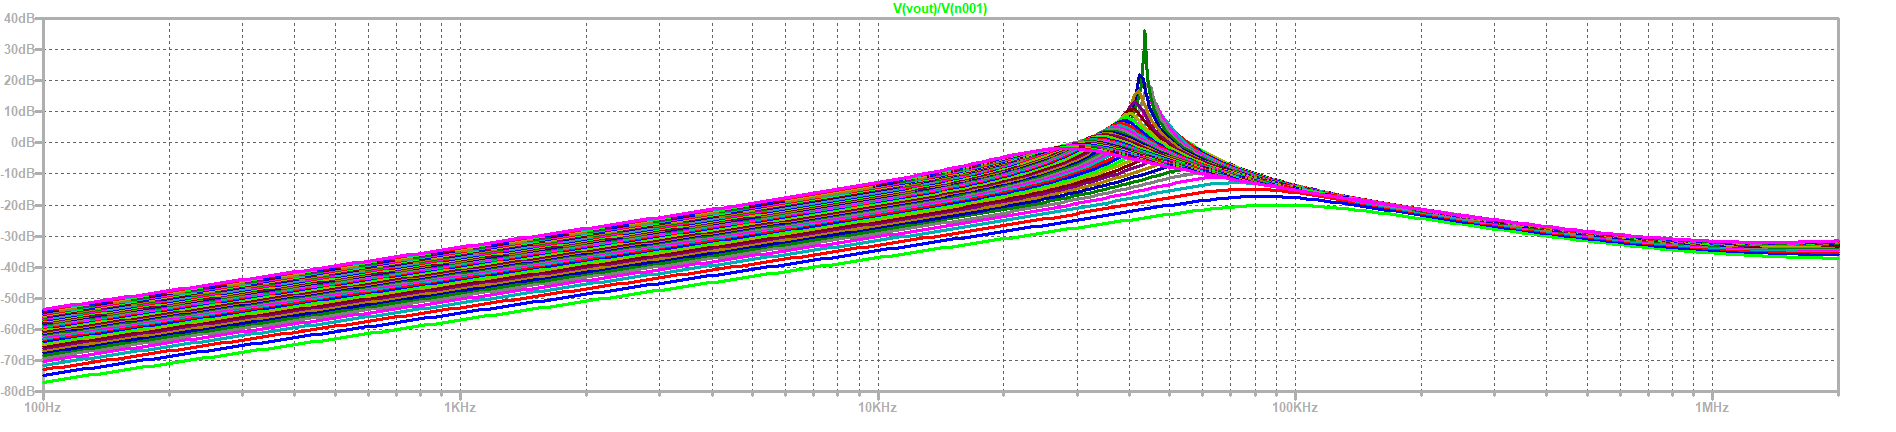
\includegraphics[width=\textwidth]{Imagenes-Ej2/presetE2.png}
	\label{fig:graph}
	\caption{Variación salida de la segunda etapa al cambiar $R_3$.}
\end{figure}
\begin{figure}[H]
	\centering
	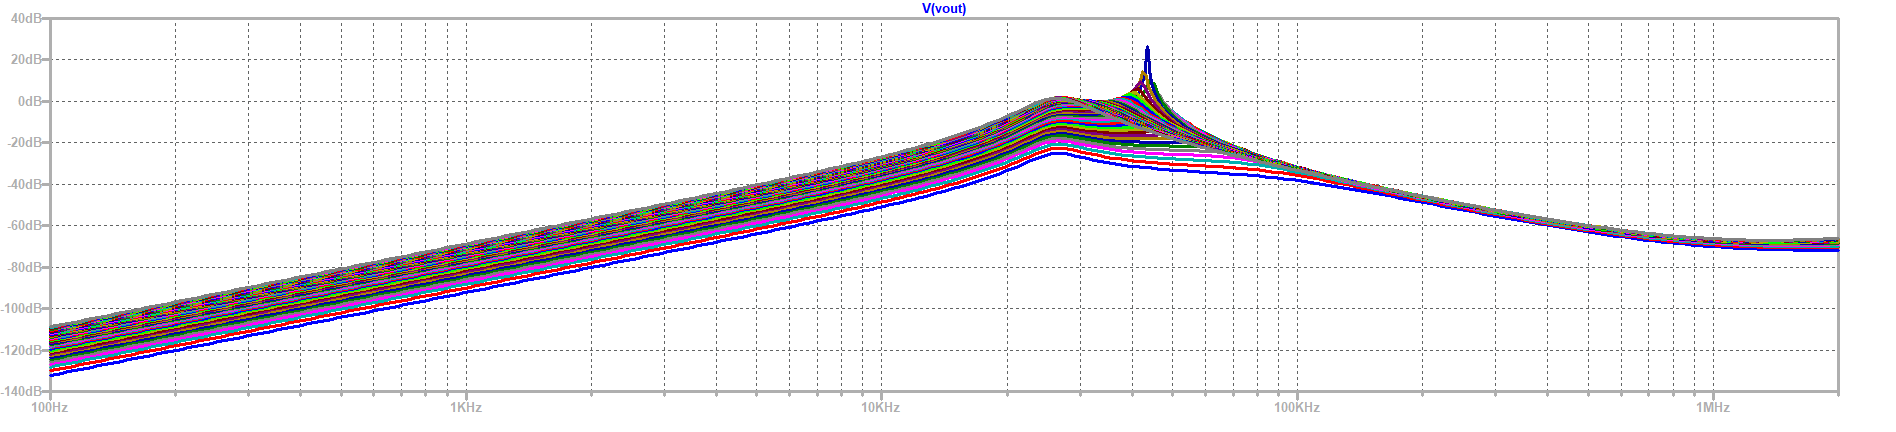
\includegraphics[width=\textwidth]{Imagenes-Ej2/presetEFE2.png}
	\label{fig:graph}
	\caption{Variación salida del filtro al cambiar $R_3$ de la segunda etapa.}
\end{figure}

En contraparte a la primer etapa, los cambios de la segunda afectan de una manera más significativa el Q, mientras que se observa lo contrario con el $\omega_0$ del circuito.

Luego se realizó un histograma de la aparición de $\omega_0$ en el análisis de Montecarlo.
\begin{figure}[H]
	\centering
	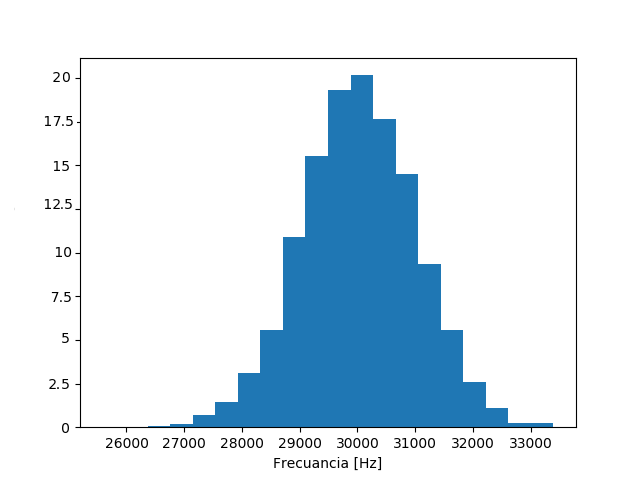
\includegraphics[width=0.7\textwidth]{Imagenes-Ej2/histW0.png}
	\label{fig:graph}
	\caption{Histograma de aparición de $\omega_0$.}
\end{figure}

\subsubsection{Filtro definitivo}
Se midió la respuesta en frecuencia del filtro obteniendo los siguientes resultados:
\begin{figure}[H]
	\centering
	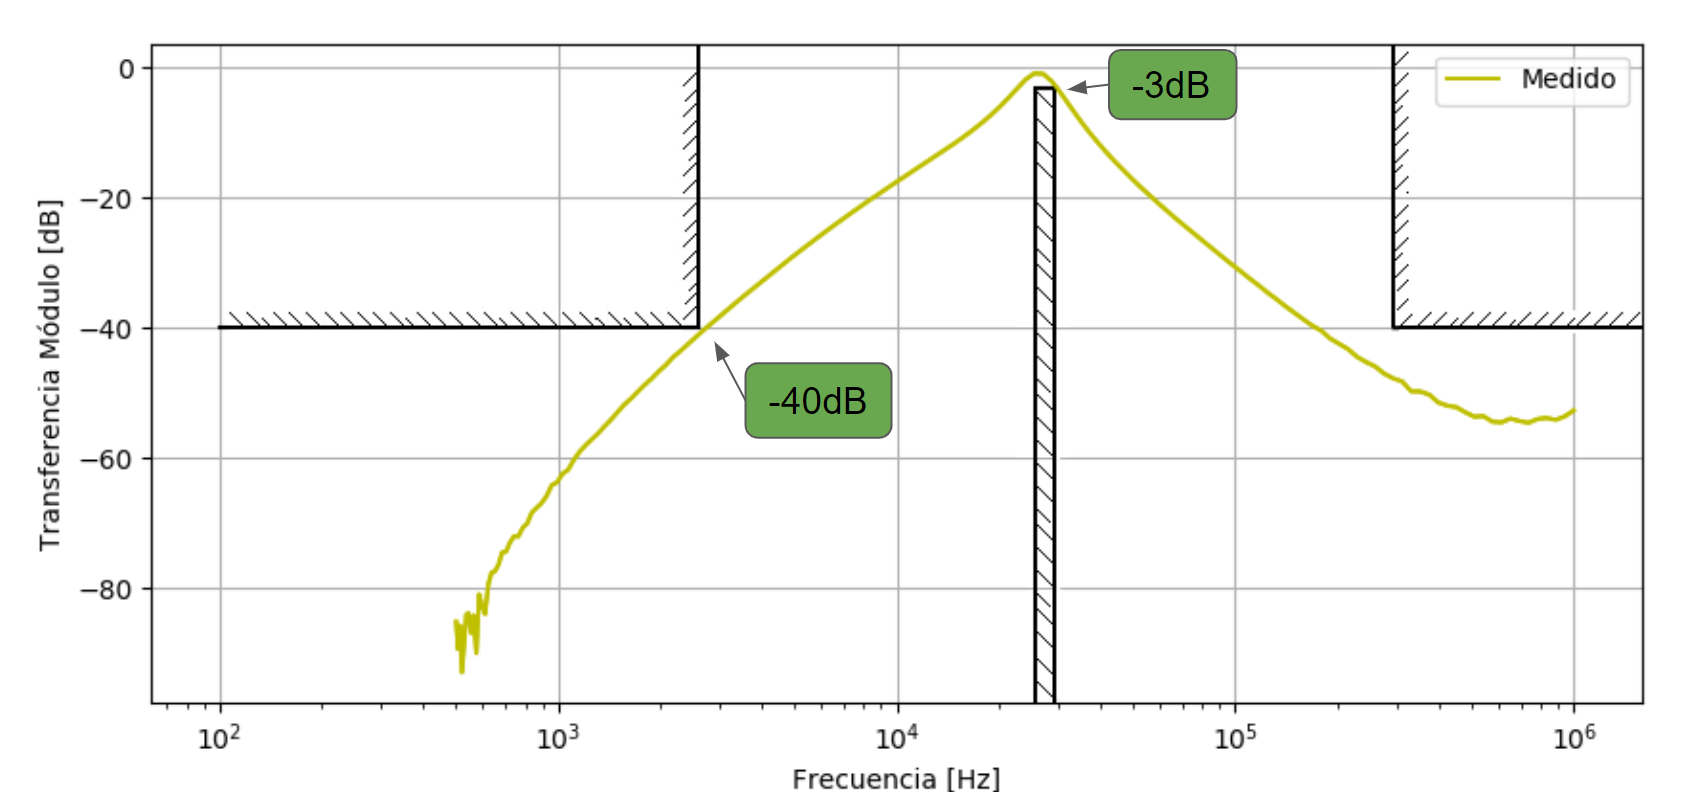
\includegraphics[width=\textwidth]{Imagenes-Ej2/BodeRauch.png}
	\caption{Bode medido en módulo.}
	\label{fig:bodemm}
\end{figure}
\begin{figure}[H]
	\centering
	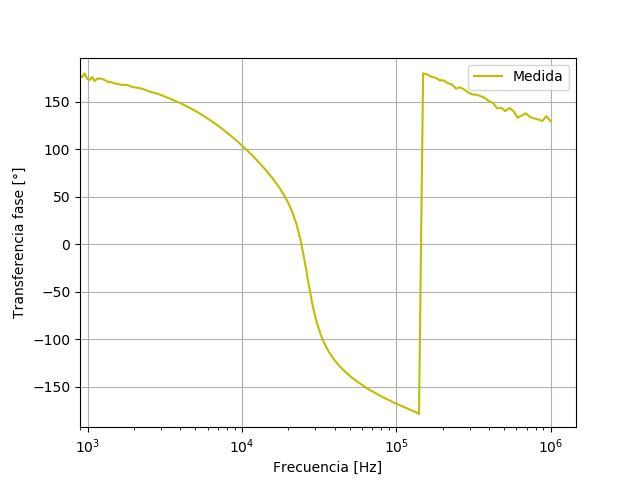
\includegraphics[width=0.7\textwidth]{Imagenes-Ej2/BodeRauchFase.png}
	\caption{Bode medido en fase.}
	\label{fig:bodemf}
\end{figure}

Luego se compararon los resultados, tanto con la simulación, como con el cálculo teórico.
\begin{figure}[H]
	\centering
	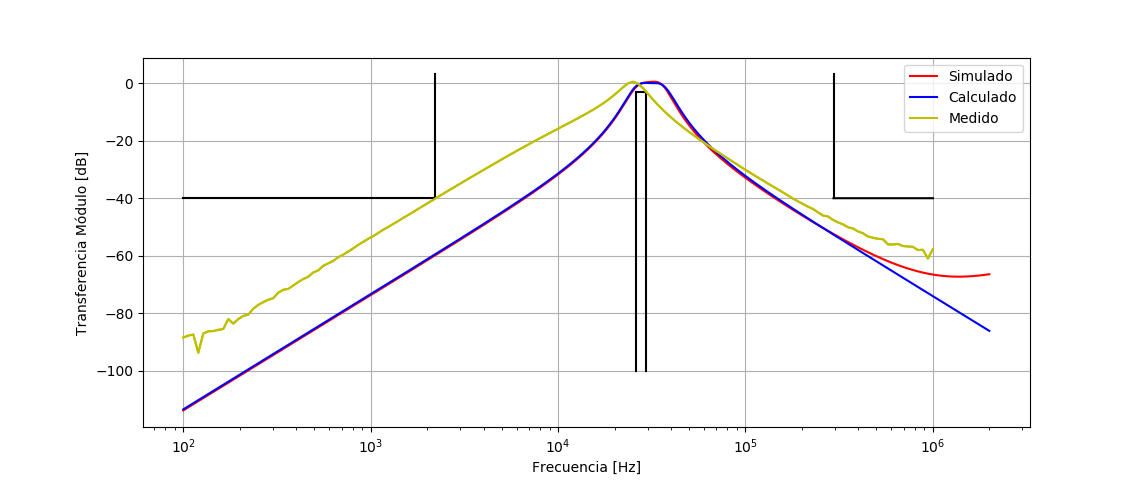
\includegraphics[width=\textwidth]{Imagenes-Ej2/BodeRauchCalcsim.png}
	\caption{Comparación de diagramas de Bode en módulo.}
	\label{fig:Bodecalcsim1}
\end{figure}
\begin{figure}[H]
	\centering
	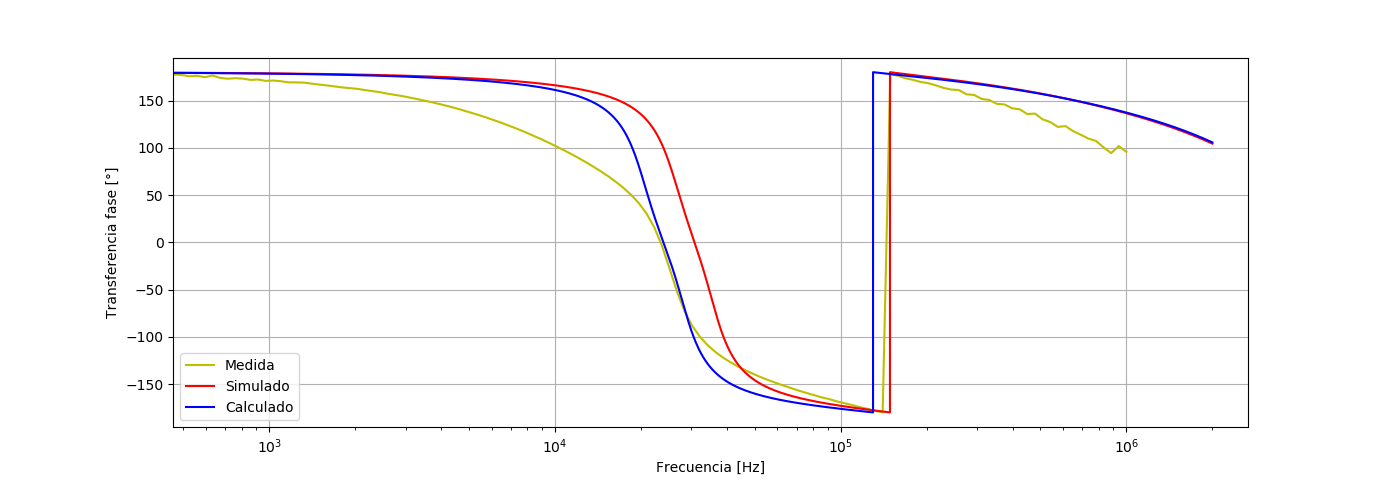
\includegraphics[width=\textwidth]{Imagenes-Ej2/BodeRauchCalcsimF.png}
	\caption{Comparación de diagramas de Bode en fase.}
	\label{fig:Bodecalcsimf1}
\end{figure}

Se puede observar como el calculado y el simulado difieren ligeramente del medido. Para solucionar esto, se colocaron presets sobre la resistencia $R_3$, ya que controla el factor Q, como se analizo previamente.
\begin{figure}[H]
	\centering
	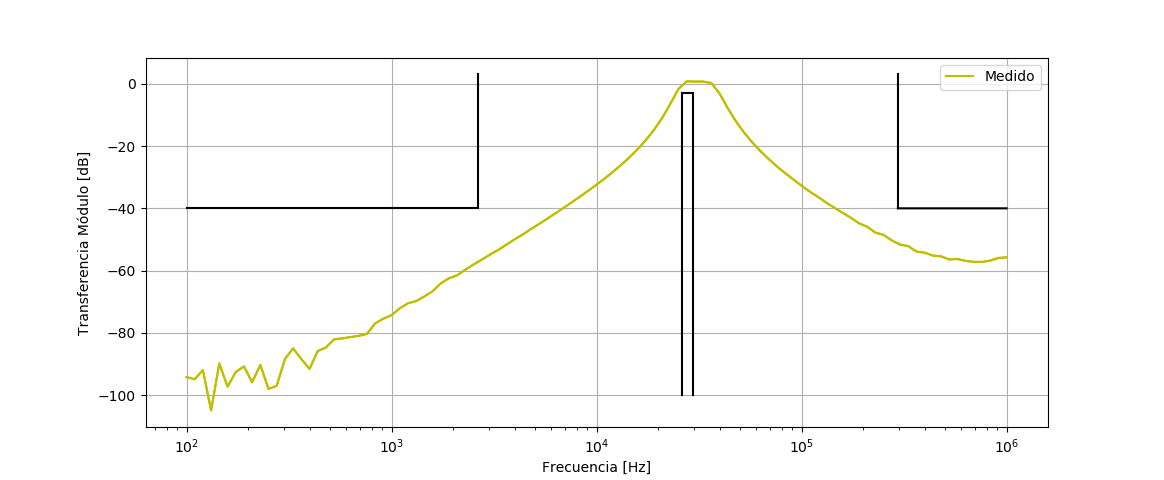
\includegraphics[width=\textwidth]{Imagenes-Ej2/BodeRauchV2.png}
	\caption{Bode medido en módulo con ajuste de $R_3$.}
	\label{fig:bodemmr}
\end{figure}
\begin{figure}[H]
	\centering
	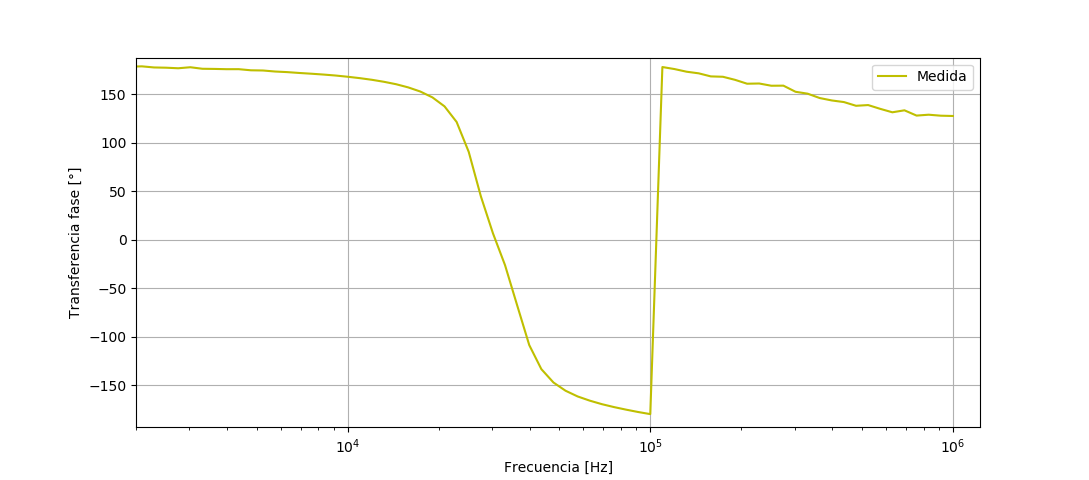
\includegraphics[width=\textwidth]{Imagenes-Ej2/BodeRauchFaseV2.png}
	\caption{Bode medido en fase con ajuste de $R_3$.}
	\label{fig:bodemfr}
\end{figure}

Debido a la calibración efectuada, el diagrama de Bode tiene una banda mucho más ancha, cumpliendo con mayor facilidad la plantilla.

\begin{figure}[H]
	\centering
	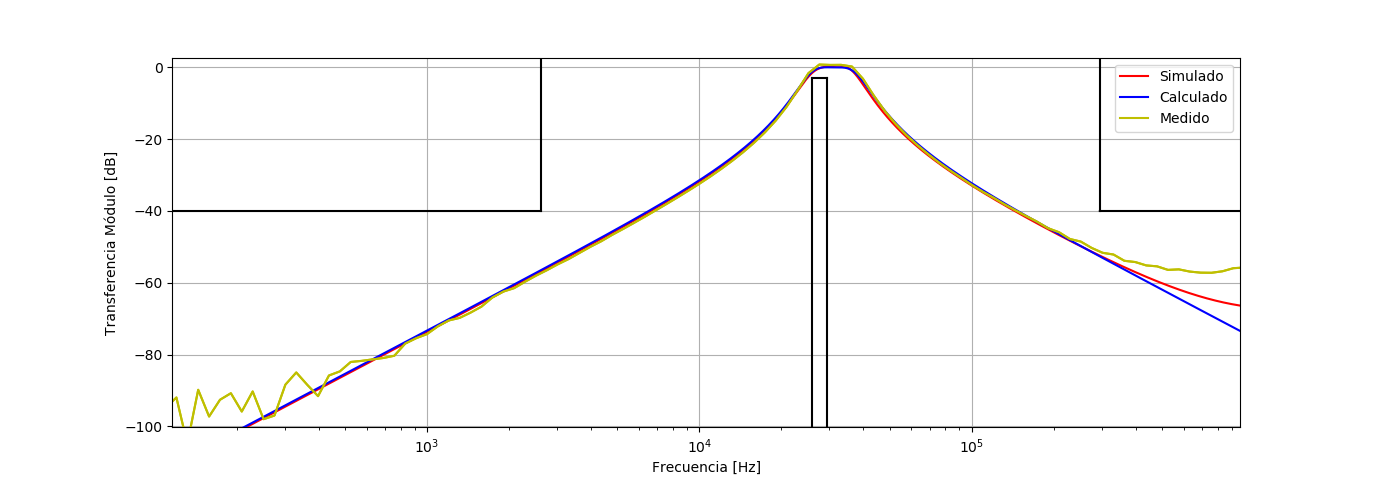
\includegraphics[width=\textwidth]{Imagenes-Ej2/BodeRauchCalcsimV2.png}
	\caption{Comparación de diagramas de Bode en módulo con ajuste de $R_3$.}
	\label{fig:Bodecalcsim2}
\end{figure}
\begin{figure}[H]
	\centering
	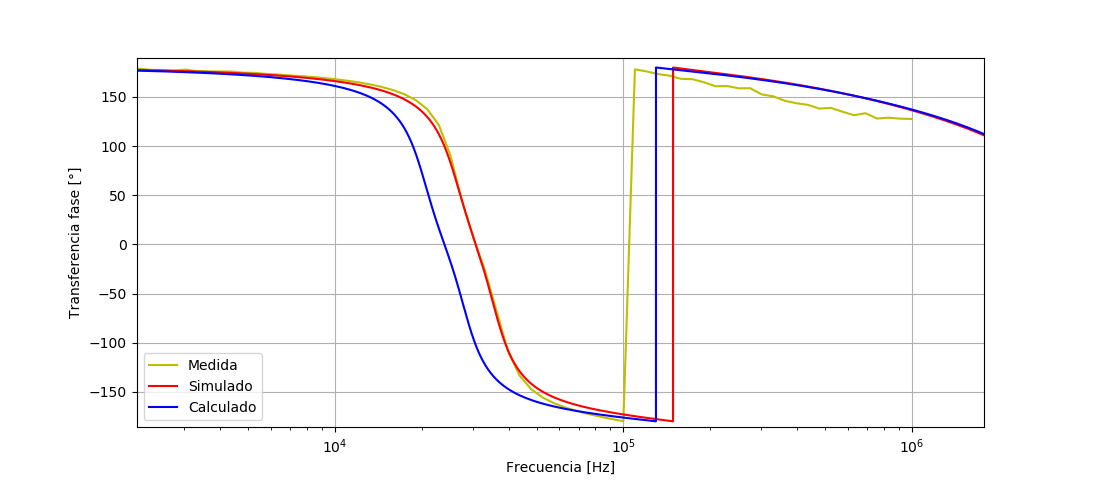
\includegraphics[width=\textwidth]{Imagenes-Ej2/BodeRauchCalcsimFV2.png}
	\caption{Comparación de diagramas de Bode en fase con ajuste de $R_3$.}
	\label{fig:Bodecalcsimf2}
\end{figure}

Es así que se observa en las Figuras (\ref{fig:Bodecalcsim2}) y (\ref{fig:Bodecalcsimf2}) como las curvas teóricas, medidas y simuladas se acoplan mucho mejor que en las Figuras (\ref{fig:Bodecalcsim1}) y (\ref{fig:Bodecalcsimf1}).

\subsection{Estabilidad}
En esta sección, se buscó lograr que la celda oscile, introduciéndole una señal cuadrada, la cual es sabido que está compuesta por un gran número de frecuencias. Es así que, variando no solo la amplitud de la misma, sino que también su frecuencia y duty-cycle, no se logró que la celda oscile. La siguiente imagen es la respuesta de la celda al escalón.
\begin{figure}[H]
	\centering
	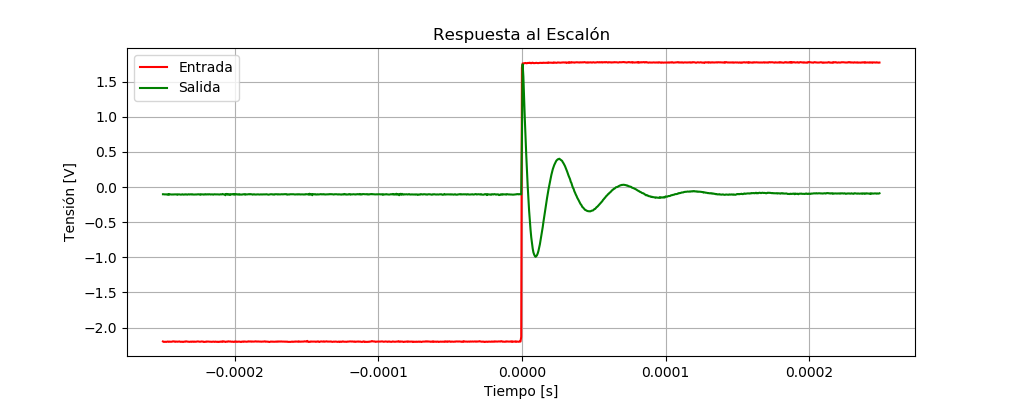
\includegraphics[width=\textwidth]{Imagenes-Ej2/Step.png}
	\label{fig:stepresponse}
	\caption{Respuesta al escalón.}
\end{figure}

\subsection{Conclusiones}
Se pudo realizar correctamente la implementación de un filtro pasa banda con la aproximación de Chebycheff mediante celdas Rauch. Una ventaja este tipo de celdas es que permite la implementación de un filtro de segundo orden con tan solo 1 operacional, mientras que por ejemplo, la celda universal, utiliza 3 de ellos. Otro punto a favor para esta es que cuenta con la capacidad de sintetizar valores de Q relativamente altos. Esto se debe a su doble realimentación, tanto negativa como positiva, mediante la utilización del Q enhancement, dando esta última una de sus desventajas, la cual consiste en la existencia de la posibilidad de que haya una oscilación en el circuito. Una cualidad a destacar es que fue de gran utilidad el uso de un preset para ajustar el Q del circuito.